\newproblem{18a}
{
	Given $f(x)=x^2-6x+5$. Identify the vertex, y-intercept, x-intercept(s), axis of symmetry, and graph the function on the graph paper and label your findings on it.\begin{onlyproblem}\begin{center}\includegraphics{fig-graphpaper.png}\end{center}\end{onlyproblem} \begin{onlysolution}\begin{center}\includegraphics{fig100-18-a-answer}\end{center}\end{onlysolution}
}
{
	\begin{tabular}{l r}
	vertex $(3, -4)$ & Add 1 pt\\
	x-intercepts $(5,0)$, $(1, 0)$ & Add 1 pt for each\\
	y-intercept $(0,5)$ & Add 1 pt\\
	Axis of Symmetry  $x=3$ & Add 1 pt\\
	Correct graph & Add 1 pt\\
	All of the points above marked on the graph & Add 2 pts\\
	\end{tabular}
}

\newproblem{18b}
{
	Given $f(x)=x^2-4x+3$. Identify the vertex, y-intercept, x-intercept(s), axis of symmetry, and graph the function on the graph paper and label your findings on it.\begin{onlyproblem}\begin{center}\includegraphics{fig-graphpaper.png}\end{center}\end{onlyproblem} \begin{onlysolution}\begin{center}\includegraphics{fig100-18-b-answer}\end{center}\end{onlysolution}
}
{
	\begin{tabular}{l r}
	vertex $(2, -1)$ & Add 1 pt\\
	x-intercepts $(1,0)$, $(3, 0)$ & Add 1 pt for each\\
	y-intercept $(0,3)$ & Add 1 pt\\
	Axis of Symmetry  $x=2$ & Add 1 pt\\
	Correct graph & Add 1 pt\\
	All of the points above marked on the graph & Add 2 pts\\
	\end{tabular}
}

\newproblem{18c}
{
	Given $f(x)=x^2-2x-3$. Identify the vertex, y-intercept, x-intercept(s), axis of symmetry, and graph the function on the graph paper and label your findings on it.\begin{onlyproblem}\begin{center}\includegraphics{fig-graphpaper.png}\end{center}\end{onlyproblem} \begin{onlysolution}\begin{center}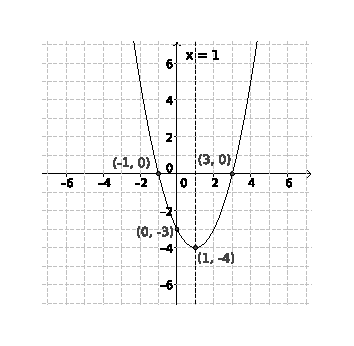
\includegraphics{fig100-18-c-answer}\end{center}\end{onlysolution}
}
{
	\begin{tabular}{l r}
	vertex $(1, -4)$ & Add 1 pt\\
	x-intercepts $(-1,0)$, $(3, 0)$ & Add 1 pt for each\\
	y-intercept $(0,-3)$ & Add 1 pt\\
	Axis of Symmetry  $x=1$ & Add 1 pt\\
	Correct graph & Add 1 pt\\
	All of the points above marked on the graph & Add 2 pts\\
	\end{tabular}
}

\newproblem{18d}
{
	Given $f(x)=x^2+2x-3$. Identify the vertex, y-intercept, x-intercept(s), axis of symmetry, and graph the function on the graph paper and label your findings on it.\begin{onlyproblem}\begin{center}\includegraphics{fig-graphpaper.png}\end{center}\end{onlyproblem} \begin{onlysolution}\begin{center}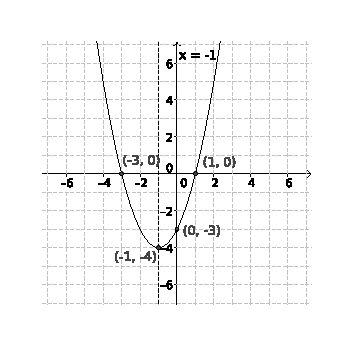
\includegraphics{fig100-18-d-answer}\end{center}\end{onlysolution}
}
{
	\begin{tabular}{l r}
	vertex $(-1, -4)$ & Add 1 pt\\
	x-intercepts $(-3,0)$, $(1, 0)$ & Add 1 pt for each\\
	y-intercept $(0,-3)$ & Add 1 pt\\
	Axis of Symmetry  $x=-1$ & Add 1 pt\\
	Correct graph & Add 1 pt\\
	All of the points above marked on the graph & Add 2 pts\\
	\end{tabular}
}
